% !TEX root = ../ds3.tex

%%%%%%%%%%%%%%%%%%%%%%%%%%%%%%%%%%%%%%%%%%%%%%%%%%%%%%%%%%%%%%%%%%%%%%%%%%%%%%%
%%%%%%%%%%%%%%%%%%%%%%%%%%%%%%%%%%%%%%%%%%%%%%%%%%%%%%%%%%%%%%%%%%%%%%%%%%%%%%%
\section{Stochastic gradient descent}
%%%%%%%%%%%%%%%%%%%%%%%%%%%%%%%%%%%%%%%%%%%%%%%%%%%%%%%%%%%%%%%%%%%%%%%%%%%%%%%
%%%%%%%%%%%%%%%%%%%%%%%%%%%%%%%%%%%%%%%%%%%%%%%%%%%%%%%%%%%%%%%%%%%%%%%%%%%%%%%


%%%%%%%%%%%%%%%%%%%%%%%%%%%%%%%%%%%%%%%%%%%%%%%%%%%%%%%%%%%%%%%%%%%%%%%%%%%%%%%
\begin{frame}{Optimization for ML: finite sum}
    Optimization in general:
    %
    \begin{align*}
        \min_{x \in \bbR^p} f(x)
    \end{align*}

    \pause

    Optimization for Machine Learning:
    %
    \begin{align*}
        \min_{x \in \bbR^p} f(x) \eqdef \sum_i^n f_i(x)
    \end{align*}

    \pause

    \begin{itemize}
        \item Can we take advantage of this \alert{finite sum} structure?
        \item In particular when the number of samples $n$ is large?
    \end{itemize}

\end{frame}
%%%%%%%%%%%%%%%%%%%%%%%%%%%%%%%%%%%%%%%%%%%%%%%%%%%%%%%%%%%%%%%%%%%%%%%%%%%%%%%

%%%%%%%%%%%%%%%%%%%%%%%%%%%%%%%%%%%%%%%%%%%%%%%%%%%%%%%%%%%%%%%%%%%%%%%%%%%%%%%
\begin{frame}{Stochastic Gradient Descent (SGD)}
    %
    \begin{itemize}
        \item Full gradient methods can be expensive
        \item \alert{Idea:} use a \alert{single gradient} $\nabla f_i(w)$ \alert{instead of of full gradient} $\sum_i^n \nabla f_i (w)$
    \end{itemize}
    %
    \vspace{2em}
    %
\begin{minipage}{0.49 \textwidth}
    \begin{algorithm}[H]
        \SetKwInOut{Input}{input}
        \SetKwInOut{Init}{init}
        \SetKwInOut{Parameter}{param}
        \caption{SGD}
        \Init{ $w = 0_{p}$, $\alpha$}
            \For{$\mathrm{iter} =1,\dots,$}
                {
                Sample $i$ in $1, \dots, n$

                \tcp{Single gradient $\nabla f_i(w)$ call}

                $w \leftarrow w - \alpha \nabla f_i (w)$

                }
    \Return{$w$}
    \end{algorithm}
\end{minipage}
%
\begin{minipage}{0.49 \textwidth}
    \begin{algorithm}[H]
        \SetKwInOut{Input}{input}
        \SetKwInOut{Init}{init}
        \SetKwInOut{Parameter}{param}
        \caption{GD}
        \Init{ $w = 0_{p}$, $\alpha$}
            \For{$\mathrm{iter} =1,\dots,$}
                {
                    \tcp{Full gradient $\nabla f (w)$ call}

                    $w \leftarrow w - \alpha \nabla f (w)$
                }
    \Return{$w$}
    \end{algorithm}
\end{minipage}
\end{frame}
%%%%%%%%%%%%%%%%%%%%%%%%%%%%%%%%%%%%%%%%%%%%%%%%%%%%%%%%%%%%%%%%%%%%%%%%%%%%%%%

%%%%%%%%%%%%%%%%%%%%%%%%%%%%%%%%%%%%%%%%%%%%%%%%%%%%%%%%%%%%%%%%%%%%%%%%%%%%%%%
\begin{frame}{SGD wit constant stepsize $\alpha$: theoretical results}
    \begin{proposition}[TODO find ref]
        If $f$ is $\mu$-strongly convex and $L$-smooth, then:
        \[
        \bbE ( \normin{w^{k} - w^*}^2 )
        \leq
        \left (
            1 - \alpha \mu
        \right)^k
        \normin{w^0 - w^*}^2
        +
        \frac{\alpha}{\mu} C
        \enspace .
        \]
    \end{proposition}
    %
    \begin{center}
        \alert{
            SGD with constant stepsize does not converge}
    \end{center}

\end{frame}
%%%%%%%%%%%%%%%%%%%%%%%%%%%%%%%%%%%%%%%%%%%%%%%%%%%%%%%%%%%%%%%%%%%%%%%%%%%%%%%

%%%%%%%%%%%%%%%%%%%%%%%%%%%%%%%%%%%%%%%%%%%%%%%%%%%%%%%%%%%%%%%%%%%%%%%%%%%%%%%
\begin{frame}{Example of SGD}
    \centering
    \only<1>{
        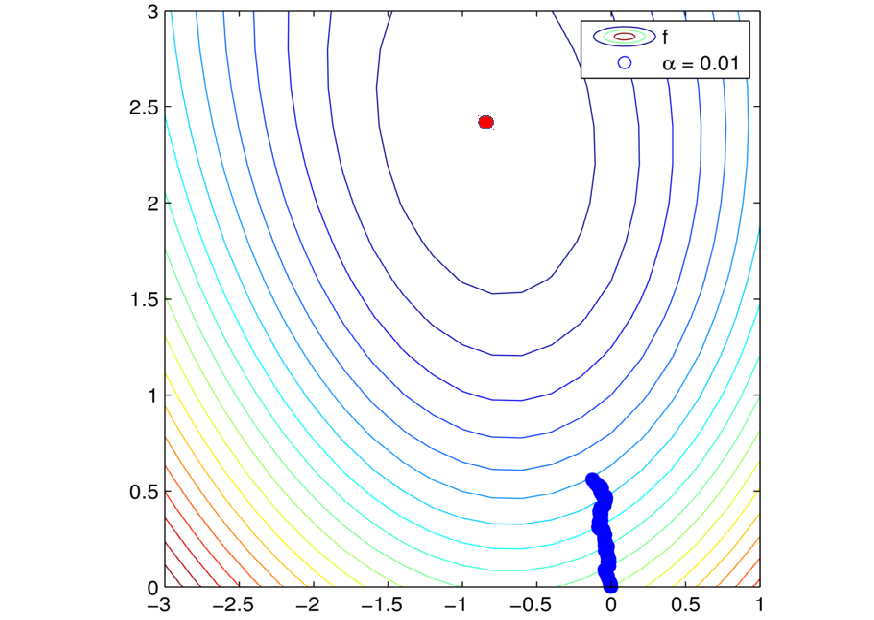
\includegraphics[width=30em]{sgd_1}
    }%
    \only<2>{
        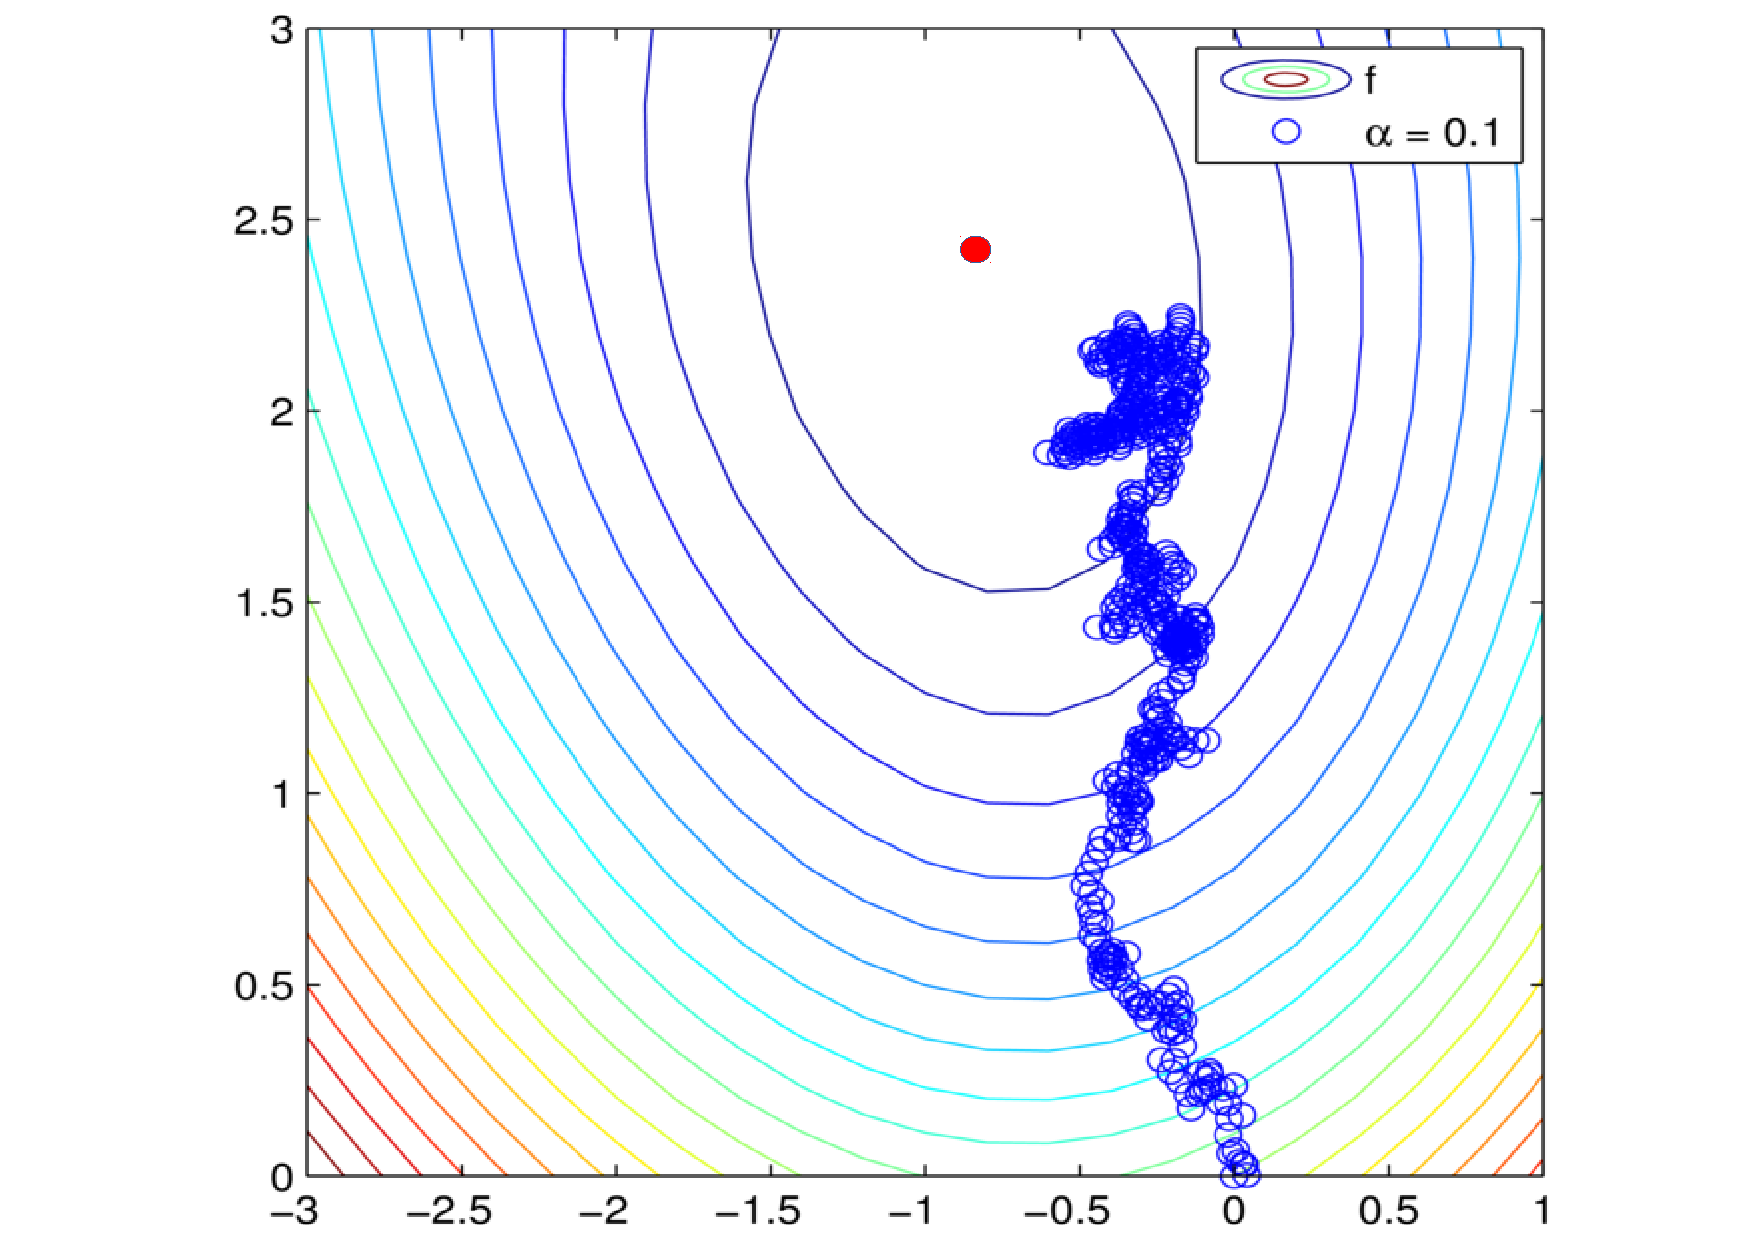
\includegraphics[width=30em]{sgd_2}
    }%
    \only<3>{
        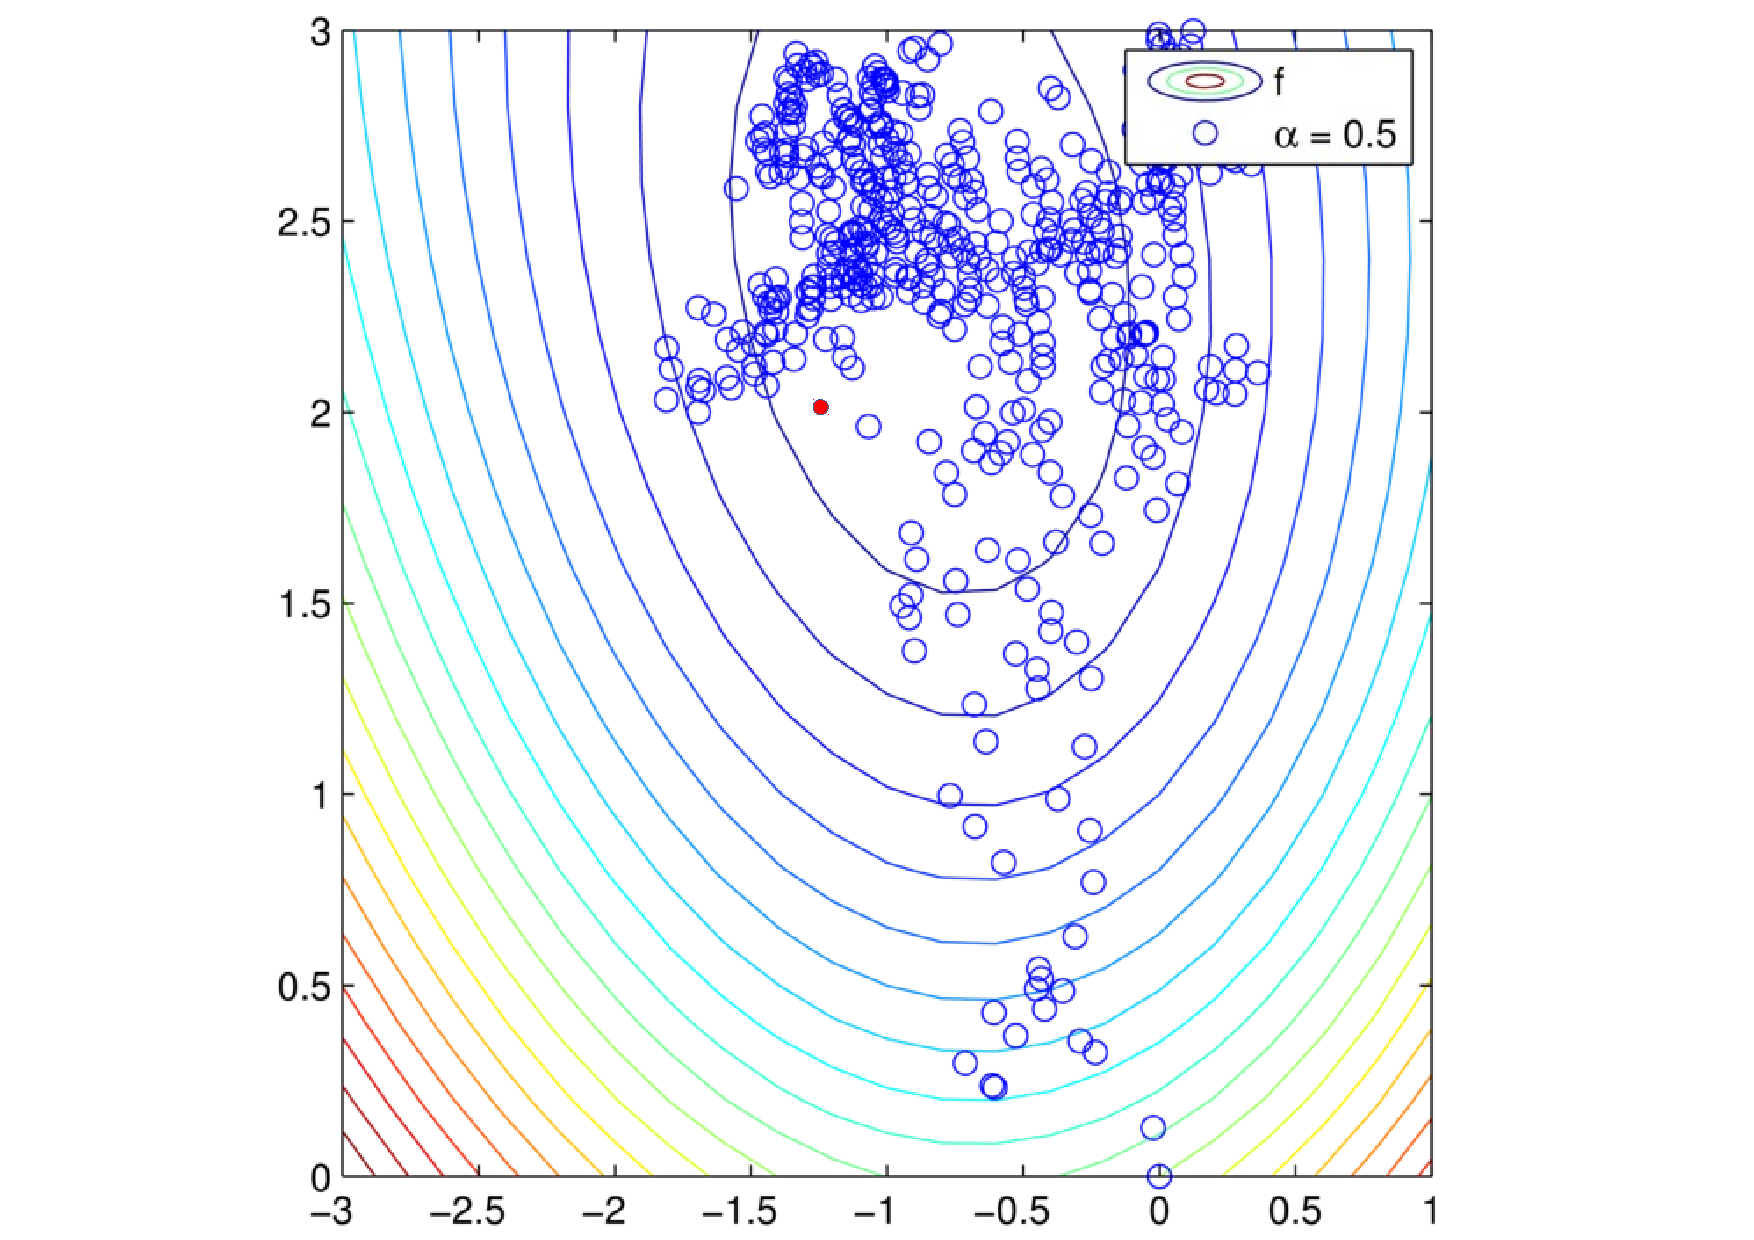
\includegraphics[width=30em]{sgd_3}
    }
    SGD on a 2D problem
\end{frame}
%%%%%%%%%%%%%%%%%%%%%%%%%%%%%%%%%%%%%%%%%%%%%%%%%%%%%%%%%%%%%%%%%%%%%%%%%%%%%%%

%%%%%%%%%%%%%%%%%%%%%%%%%%%%%%%%%%%%%%%%%%%%%%%%%%%%%%%%%%%%%%%%%%%%%%%%%%%%%%%
\begin{frame}{Exercise: lab3 'stochastic gradient descent'}
    Your turn!

    \begin{itemize}
        \item  Play with SGD to gain insight: make $n$ vary!
        \item Play with the regularization parameter $\lambda$
        \item Play with the correlation of the data to see what's happening
    \end{itemize}

    \vspace{2em}

    Reminders!
    \begin{itemize}
        \item In all the labs the main algorithm is already coded, and we propose you to add little modifications
        \item All the solutions are in the solutions folder
    \end{itemize}
\end{frame}
%%%%%%%%%%%%%%%%%%%%%%%%%%%%%%%%%%%%%%%%%%%%%%%%%%%%%%%%%%%%%%%%%%%%%%%%%%%%%%%
